%last updated in April 2002 by Antje Endemann

\documentclass[runningheads]{llncs}
%In order to omit page numbers and running heads
%please use the following line instead of the first command line:
%\documentclass{llncs}.
%Furthermore change the line \pagestyle{headings} to
%\pagestyle{empty}.
\usepackage{graphicx}
\usepackage{url}
\usepackage{color}
\usepackage{amsmath}
\newcommand{\argmin}{\operatornamewithlimits{argmin}}
\newcommand {\afbnote} [1] {{\bf \textcolor{red}{(#1)}}}
\newcommand {\ericnote} [1] {{\bf \textcolor{magenta}{(#1)}}}
\newcommand {\PnP} {P$n$P}
\newcommand {\EPnP} {EP$n$P}
% Psfig/TeX 
\def\PsfigVersion{1.10}
\def\setDriver{\DvipsDriver} % \DvipsDriver or \OzTeXDriver
%
% All software, documentation, and related files in this distribution of
% psfig/tex are Copyright 1993 Trevor J. Darrell
%
% Permission is granted for use and non-profit distribution of psfig/tex 
% providing that this notice is clearly maintained. The right to
% distribute any portion of psfig/tex for profit or as part of any commercial
% product is specifically reserved for the author(s) of that portion.
%
% To use with LaTeX, use \documentstyle[psfig,...]{...}
% To use with TeX, use \input psfig.sty
%
% Bugs and improvements to trevor@media.mit.edu.
%
% Thanks to Ned Batchelder, Greg Hager (GDH), J. Daniel Smith (JDS),
% Tom Rokicki (TR), Robert Russell (RR), George V. Reilly (GVR),
% Ken McGlothlen (KHC), Baron Grey (BG), Gerhard Tobermann (GT).
% and all others who have contributed code and comments to this project!
%
% ======================================================================
% Modification History:
%
%  9 Oct 1990   JDS	used more robust bbox reading code from Tom Rokicki
% 29 Mar 1991   JDS	implemented rotation= option
% 25 Jun 1991   RR	if bb specified on cmd line don't check
%			for .ps file.
%  3 Jul 1991	JDS	check if file already read in once
%  4 Sep 1991	JDS	fixed incorrect computation of rotated
%			bounding box
% 25 Sep 1991	GVR	expanded synopsis of \psfig
% 14 Oct 1991	JDS	\fbox code from LaTeX so \psdraft works with TeX
%			changed \typeout to \ps@typeout
% 17 Oct 1991	JDS	added \psscalefirst and \psrotatefirst
% 23 Jun 1993   KHC     ``doclip'' must appear before ``rotate''
% 27 Oct 1993   TJD	removed printing of filename to avoid 
%			underscore problems. changed \frame to \fbox.
%			Added OzTeX support from BG. Added new
%			figure search path code from GT.
%
% ======================================================================
%
% Command synopsis:
%
% \psdraft	draws an outline box, but doesn't include the figure
%		in the DVI file.  Useful for previewing.
%
% \psfull	includes the figure in the DVI file (default).
%
% \psscalefirst width= or height= specifies the size of the figure
% 		before rotation.
% \psrotatefirst (default) width= or height= specifies the size of the
% 		 figure after rotation.  Asymetric figures will
% 		 appear to shrink.
%
% \psfigurepath{dir:dir:...}  sets the path to search for the figure
%
% \psfig
% usage: \psfig{file=, figure=, height=, width=,
%			bbllx=, bblly=, bburx=, bbury=,
%			rheight=, rwidth=, clip=, angle=, silent=}
%
%	"file" is the filename.  If no path name is specified and the
%		file is not found in the current directory,
%		it will be looked for in directory \psfigurepath.
%	"figure" is a synonym for "file".
%	By default, the width and height of the figure are taken from
%		the BoundingBox of the figure.
%	If "width" is specified, the figure is scaled so that it has
%		the specified width.  Its height changes proportionately.
%	If "height" is specified, the figure is scaled so that it has
%		the specified height.  Its width changes proportionately.
%	If both "width" and "height" are specified, the figure is scaled
%		anamorphically.
%	"bbllx", "bblly", "bburx", and "bbury" control the PostScript
%		BoundingBox.  If these four values are specified
%               *before* the "file" option, the PSFIG will not try to
%               open the PostScript file.
%	"rheight" and "rwidth" are the reserved height and width
%		of the figure, i.e., how big TeX actually thinks
%		the figure is.  They default to "width" and "height".
%	The "clip" option ensures that no portion of the figure will
%		appear outside its BoundingBox.  "clip=" is a switch and
%		takes no value, but the `=' must be present.
%	The "angle" option specifies the angle of rotation (degrees, ccw).
%	The "silent" option makes \psfig work silently.
%
% ======================================================================
% check to see if macros already loaded in (maybe some other file says
% "\input psfig") ...
\ifx\undefined\psfig\else\endinput\fi
%
% from a suggestion by eijkhout@csrd.uiuc.edu to allow
% loading as a style file. Changed to avoid problems
% with amstex per suggestion by jbence@math.ucla.edu

\let\LaTeXAtSign=\@
\let\@=\relax
\edef\psfigRestoreAt{\catcode`\@=\number\catcode`@\relax}
%\edef\psfigRestoreAt{\catcode`@=\number\catcode`@\relax}
\catcode`\@=11\relax
\newwrite\@unused
\def\ps@typeout#1{{\let\protect\string\immediate\write\@unused{#1}}}

\def\DvipsDriver{
	\ps@typeout{psfig/tex \PsfigVersion -dvips}
\def\PsfigSpecials{\DvipsSpecials} 	\def\ps@dir{/}
\def\ps@predir{} }
\def\OzTeXDriver{
	\ps@typeout{psfig/tex \PsfigVersion -oztex}
	\def\PsfigSpecials{\OzTeXSpecials}
	\def\ps@dir{:}
	\def\ps@predir{:}
	\catcode`\^^J=5
}

%% Here's how you define your figure path.  Should be set up with null
%% default and a user useable definition.

\def\figurepath{./:}
\def\psfigurepath#1{\edef\figurepath{#1:}}

%%% inserted for Searching Unixpaths
%%% (the path must end with :)
%%% (call: \DoPaths\figurepath )
%%%------------------------------------------------------
\def\DoPaths#1{\expandafter\EachPath#1\stoplist}
%
\def\leer{}
\def\EachPath#1:#2\stoplist{% #1 part of the list (delimiter :)
  \ExistsFile{#1}{\SearchedFile}
  \ifx#2\leer
  \else
    \expandafter\EachPath#2\stoplist
  \fi}
%
% exists the file (does not work for directories!)
%
\def\ps@dir{/}
\def\ExistsFile#1#2{%
   \openin1=\ps@predir#1\ps@dir#2
   \ifeof1
       \closein1
       %\ps@typeout{...not: \ps@predir#1\ps@dir#2}
   \else
       \closein1
       %\ps@typeout{...in:  \ps@predir#1\ps@dir#2}
        \ifx\ps@founddir\leer
          %\ps@typeout{set founddir #1}
           \edef\ps@founddir{#1}
        \fi
   \fi}
%------------------------------------------------------
%
% Get dir in path or error
%
\def\get@dir#1{%
  \def\ps@founddir{}
  \def\SearchedFile{#1}
  \DoPaths\figurepath
%  \fi
}
%------------------------------------------------------
%%% END of Searching Unixpaths


%
% @psdo control structure -- similar to Latex @for.
% I redefined these with different names so that psfig can
% be used with TeX as well as LaTeX, and so that it will not 
% be vunerable to future changes in LaTeX's internal
% control structure,
%
\def\@nnil{\@nil}
\def\@empty{}
\def\@psdonoop#1\@@#2#3{}
\def\@psdo#1:=#2\do#3{\edef\@psdotmp{#2}\ifx\@psdotmp\@empty \else
    \expandafter\@psdoloop#2,\@nil,\@nil\@@#1{#3}\fi}
\def\@psdoloop#1,#2,#3\@@#4#5{\def#4{#1}\ifx #4\@nnil \else
       #5\def#4{#2}\ifx #4\@nnil \else#5\@ipsdoloop #3\@@#4{#5}\fi\fi}
\def\@ipsdoloop#1,#2\@@#3#4{\def#3{#1}\ifx #3\@nnil 
       \let\@nextwhile=\@psdonoop \else
      #4\relax\let\@nextwhile=\@ipsdoloop\fi\@nextwhile#2\@@#3{#4}}
\def\@tpsdo#1:=#2\do#3{\xdef\@psdotmp{#2}\ifx\@psdotmp\@empty \else
    \@tpsdoloop#2\@nil\@nil\@@#1{#3}\fi}
\def\@tpsdoloop#1#2\@@#3#4{\def#3{#1}\ifx #3\@nnil 
       \let\@nextwhile=\@psdonoop \else
      #4\relax\let\@nextwhile=\@tpsdoloop\fi\@nextwhile#2\@@#3{#4}}
% 
% \fbox is defined in latex.tex; so if \fbox is undefined, assume that
% we are not in LaTeX.
% Perhaps this could be done better???
\ifx\undefined\fbox
% \fbox code from modified slightly from LaTeX
\newdimen\fboxrule
\newdimen\fboxsep
\newdimen\ps@tempdima
\newbox\ps@tempboxa
\fboxsep = 3pt
\fboxrule = .4pt
\long\def\fbox#1{\leavevmode\setbox\ps@tempboxa\hbox{#1}\ps@tempdima\fboxrule
    \advance\ps@tempdima \fboxsep \advance\ps@tempdima \dp\ps@tempboxa
   \hbox{\lower \ps@tempdima\hbox
  {\vbox{\hrule height \fboxrule
          \hbox{\vrule width \fboxrule \hskip\fboxsep
          \vbox{\vskip\fboxsep \box\ps@tempboxa\vskip\fboxsep}\hskip 
                 \fboxsep\vrule width \fboxrule}
                 \hrule height \fboxrule}}}}
\fi
%
%%%%%%%%%%%%%%%%%%%%%%%%%%%%%%%%%%%%%%%%%%%%%%%%%%%%%%%%%%%%%%%%%%%
% file reading stuff from epsf.tex
%   EPSF.TEX macro file:
%   Written by Tomas Rokicki of Radical Eye Software, 29 Mar 1989.
%   Revised by Don Knuth, 3 Jan 1990.
%   Revised by Tomas Rokicki to accept bounding boxes with no
%      space after the colon, 18 Jul 1990.
%   Portions modified/removed for use in PSFIG package by
%      J. Daniel Smith, 9 October 1990.
%
\newread\ps@stream
\newif\ifnot@eof       % continue looking for the bounding box?
\newif\if@noisy        % report what you're making?
\newif\if@atend        % %%BoundingBox: has (at end) specification
\newif\if@psfile       % does this look like a PostScript file?
%
% PostScript files should start with `%!'
%
{\catcode`\%=12\global\gdef\epsf@start{%!}}
\def\epsf@PS{PS}
%
\def\epsf@getbb#1{%
%
%   The first thing we need to do is to open the
%   PostScript file, if possible.
%
\openin\ps@stream=\ps@predir#1
\ifeof\ps@stream\ps@typeout{Error, File #1 not found}\else
%
%   Okay, we got it. Now we'll scan lines until we find one that doesn't
%   start with %. We're looking for the bounding box comment.
%
   {\not@eoftrue \chardef\other=12
    \def\do##1{\catcode`##1=\other}\dospecials \catcode`\ =10
    \loop
       \if@psfile
	  \read\ps@stream to \epsf@fileline
       \else{
	  \obeyspaces
          \read\ps@stream to \epsf@tmp\global\let\epsf@fileline\epsf@tmp}
       \fi
       \ifeof\ps@stream\not@eoffalse\else
%
%   Check the first line for `%!'.  Issue a warning message if its not
%   there, since the file might not be a PostScript file.
%
       \if@psfile\else
       \expandafter\epsf@test\epsf@fileline:. \\%
       \fi
%
%   We check to see if the first character is a % sign;
%   if so, we look further and stop only if the line begins with
%   `%%BoundingBox:' and the `(atend)' specification was not found.
%   That is, the only way to stop is when the end of file is reached,
%   or a `%%BoundingBox: llx lly urx ury' line is found.
%
          \expandafter\epsf@aux\epsf@fileline:. \\%
       \fi
   \ifnot@eof\repeat
   }\closein\ps@stream\fi}%
%
% This tests if the file we are reading looks like a PostScript file.
%
\long\def\epsf@test#1#2#3:#4\\{\def\epsf@testit{#1#2}
			\ifx\epsf@testit\epsf@start\else
\ps@typeout{Warning! File does not start with `\epsf@start'.  It may not be a PostScript file.}
			\fi
			\@psfiletrue} % don't test after 1st line
%
%   We still need to define the tricky \epsf@aux macro. This requires
%   a couple of magic constants for comparison purposes.
%
{\catcode`\%=12\global\let\epsf@percent=%\global\def\epsf@bblit{%BoundingBox}}
%
%
%   So we're ready to check for `%BoundingBox:' and to grab the
%   values if they are found.  We continue searching if `(at end)'
%   was found after the `%BoundingBox:'.
%
\long\def\epsf@aux#1#2:#3\\{\ifx#1\epsf@percent
   \def\epsf@testit{#2}\ifx\epsf@testit\epsf@bblit
	\@atendfalse
        \epsf@atend #3 . \\%
	\if@atend	
	   \if@verbose{
		\ps@typeout{psfig: found `(atend)'; continuing search}
	   }\fi
        \else
        \epsf@grab #3 . . . \\%
        \not@eoffalse
        \global\no@bbfalse
        \fi
   \fi\fi}%
%
%   Here we grab the values and stuff them in the appropriate definitions.
%
\def\epsf@grab #1 #2 #3 #4 #5\\{%
   \global\def\epsf@llx{#1}\ifx\epsf@llx\empty
      \epsf@grab #2 #3 #4 #5 .\\\else
   \global\def\epsf@lly{#2}%
   \global\def\epsf@urx{#3}\global\def\epsf@ury{#4}\fi}%
%
% Determine if the stuff following the %%BoundingBox is `(atend)'
% J. Daniel Smith.  Copied from \epsf@grab above.
%
\def\epsf@atendlit{(atend)} 
\def\epsf@atend #1 #2 #3\\{%
   \def\epsf@tmp{#1}\ifx\epsf@tmp\empty
      \epsf@atend #2 #3 .\\\else
   \ifx\epsf@tmp\epsf@atendlit\@atendtrue\fi\fi}


% End of file reading stuff from epsf.tex
%%%%%%%%%%%%%%%%%%%%%%%%%%%%%%%%%%%%%%%%%%%%%%%%%%%%%%%%%%%%%%%%%%%

%%%%%%%%%%%%%%%%%%%%%%%%%%%%%%%%%%%%%%%%%%%%%%%%%%%%%%%%%%%%%%%%%%%
% trigonometry stuff from "trig.tex"
\chardef\psletter = 11 % won't conflict with \begin{letter} now...
\chardef\other = 12

\newif \ifdebug %%% turn me on to see TeX hard at work ...
\newif\ifc@mpute %%% don't need to compute some values
\c@mputetrue % but assume that we do

\let\then = \relax
\def\r@dian{pt }
\let\r@dians = \r@dian
\let\dimensionless@nit = \r@dian
\let\dimensionless@nits = \dimensionless@nit
\def\internal@nit{sp }
\let\internal@nits = \internal@nit
\newif\ifstillc@nverging
\def \Mess@ge #1{\ifdebug \then \message {#1} \fi}

{ %%% Things that need abnormal catcodes %%%
	\catcode `\@ = \psletter
	\gdef \nodimen {\expandafter \n@dimen \the \dimen}
	\gdef \term #1 #2 #3%
	       {\edef \t@ {\the #1}%%% freeze parameter 1 (count, by value)
		\edef \t@@ {\expandafter \n@dimen \the #2\r@dian}%
				   %%% freeze parameter 2 (dimen, by value)
		\t@rm {\t@} {\t@@} {#3}%
	       }
	\gdef \t@rm #1 #2 #3%
	       {{%
		\count 0 = 0
		\dimen 0 = 1 \dimensionless@nit
		\dimen 2 = #2\relax
		\Mess@ge {Calculating term #1 of \nodimen 2}%
		\loop
		\ifnum	\count 0 < #1
		\then	\advance \count 0 by 1
			\Mess@ge {Iteration \the \count 0 \space}%
			\Multiply \dimen 0 by {\dimen 2}%
			\Mess@ge {After multiplication, term = \nodimen 0}%
			\Divide \dimen 0 by {\count 0}%
			\Mess@ge {After division, term = \nodimen 0}%
		\repeat
		\Mess@ge {Final value for term #1 of 
				\nodimen 2 \space is \nodimen 0}%
		\xdef \Term {#3 = \nodimen 0 \r@dians}%
		\aftergroup \Term
	       }}
	\catcode `\p = \other
	\catcode `\t = \other
	\gdef \n@dimen #1pt{#1} %%% throw away the ``pt''
}

\def \Divide #1by #2{\divide #1 by #2} %%% just a synonym

\def \Multiply #1by #2%%% allows division of a dimen by a dimen
       {{%%% should really freeze parameter 2 (dimen, passed by value)
	\count 0 = #1\relax
	\count 2 = #2\relax
	\count 4 = 65536
	\Mess@ge {Before scaling, count 0 = \the \count 0 \space and
			count 2 = \the \count 2}%
	\ifnum	\count 0 > 32767 %%% do our best to avoid overflow
	\then	\divide \count 0 by 4
		\divide \count 4 by 4
	\else	\ifnum	\count 0 < -32767
		\then	\divide \count 0 by 4
			\divide \count 4 by 4
		\else
		\fi
	\fi
	\ifnum	\count 2 > 32767 %%% while retaining reasonable accuracy
	\then	\divide \count 2 by 4
		\divide \count 4 by 4
	\else	\ifnum	\count 2 < -32767
		\then	\divide \count 2 by 4
			\divide \count 4 by 4
		\else
		\fi
	\fi
	\multiply \count 0 by \count 2
	\divide \count 0 by \count 4
	\xdef \product {#1 = \the \count 0 \internal@nits}%
	\aftergroup \product
       }}

\def\r@duce{\ifdim\dimen0 > 90\r@dian \then   % sin(x+90) = sin(180-x)
		\multiply\dimen0 by -1
		\advance\dimen0 by 180\r@dian
		\r@duce
	    \else \ifdim\dimen0 < -90\r@dian \then  % sin(-x) = sin(360+x)
		\advance\dimen0 by 360\r@dian
		\r@duce
		\fi
	    \fi}

\def\Sine#1%
       {{%
	\dimen 0 = #1 \r@dian
	\r@duce
	\ifdim\dimen0 = -90\r@dian \then
	   \dimen4 = -1\r@dian
	   \c@mputefalse
	\fi
	\ifdim\dimen0 = 90\r@dian \then
	   \dimen4 = 1\r@dian
	   \c@mputefalse
	\fi
	\ifdim\dimen0 = 0\r@dian \then
	   \dimen4 = 0\r@dian
	   \c@mputefalse
	\fi
%
	\ifc@mpute \then
        	% convert degrees to radians
		\divide\dimen0 by 180
		\dimen0=3.141592654\dimen0
%
		\dimen 2 = 3.1415926535897963\r@dian %%% a well-known constant
		\divide\dimen 2 by 2 %%% we only deal with -pi/2 : pi/2
		\Mess@ge {Sin: calculating Sin of \nodimen 0}%
		\count 0 = 1 %%% see power-series expansion for sine
		\dimen 2 = 1 \r@dian %%% ditto
		\dimen 4 = 0 \r@dian %%% ditto
		\loop
			\ifnum	\dimen 2 = 0 %%% then we've done
			\then	\stillc@nvergingfalse 
			\else	\stillc@nvergingtrue
			\fi
			\ifstillc@nverging %%% then calculate next term
			\then	\term {\count 0} {\dimen 0} {\dimen 2}%
				\advance \count 0 by 2
				\count 2 = \count 0
				\divide \count 2 by 2
				\ifodd	\count 2 %%% signs alternate
				\then	\advance \dimen 4 by \dimen 2
				\else	\advance \dimen 4 by -\dimen 2
				\fi
		\repeat
	\fi		
			\xdef \sine {\nodimen 4}%
       }}

% Now the Cosine can be calculated easily by calling \Sine
\def\Cosine#1{\ifx\sine\UnDefined\edef\Savesine{\relax}\else
		             \edef\Savesine{\sine}\fi
	{\dimen0=#1\r@dian\advance\dimen0 by 90\r@dian
	 \Sine{\nodimen 0}
	 \xdef\cosine{\sine}
	 \xdef\sine{\Savesine}}}	      
% end of trig stuff
%%%%%%%%%%%%%%%%%%%%%%%%%%%%%%%%%%%%%%%%%%%%%%%%%%%%%%%%%%%%%%%%%%%%

\def\psdraft{
	\def\@psdraft{0}
	%\ps@typeout{draft level now is \@psdraft \space . }
}
\def\psfull{
	\def\@psdraft{100}
	%\ps@typeout{draft level now is \@psdraft \space . }
}

\psfull

\newif\if@scalefirst
\def\psscalefirst{\@scalefirsttrue}
\def\psrotatefirst{\@scalefirstfalse}
\psrotatefirst

\newif\if@draftbox
\def\psnodraftbox{
	\@draftboxfalse
}
\def\psdraftbox{
	\@draftboxtrue
}
\@draftboxtrue

\newif\if@prologfile
\newif\if@postlogfile
\def\pssilent{
	\@noisyfalse
}
\def\psnoisy{
	\@noisytrue
}
\psnoisy
%%% These are for the option list.
%%% A specification of the form a = b maps to calling \@p@@sa{b}
\newif\if@bbllx
\newif\if@bblly
\newif\if@bburx
\newif\if@bbury
\newif\if@height
\newif\if@width
\newif\if@rheight
\newif\if@rwidth
\newif\if@angle
\newif\if@clip
\newif\if@verbose
\def\@p@@sclip#1{\@cliptrue}
%
%
\newif\if@decmpr
%
\def\@p@@sfigure#1{\def\@p@sfile{null}\def\@p@sbbfile{null}\@decmprfalse
   % look directly for file (e.g. absolute path)
   \openin1=\ps@predir#1
   \ifeof1
	\closein1
	% failed, search directories for file
	\get@dir{#1}
	\ifx\ps@founddir\leer
		% failed, search directly for file.bb
		\openin1=\ps@predir#1.bb
		\ifeof1
			\closein1
			% failed, search directories for file.bb
			\get@dir{#1.bb}
			\ifx\ps@founddir\leer
				% failed, lose.
				\ps@typeout{Can't find #1 in \figurepath}
			\else
				% found file.bb in search dir
				\@decmprtrue
				\def\@p@sfile{\ps@founddir\ps@dir#1}
				\def\@p@sbbfile{\ps@founddir\ps@dir#1.bb}
			\fi
		\else
			\closein1
			%found file.bb directly
			\@decmprtrue
			\def\@p@sfile{#1}
			\def\@p@sbbfile{#1.bb}
		\fi
	\else
		% found file in search dir
		\def\@p@sfile{\ps@founddir\ps@dir#1}
		\def\@p@sbbfile{\ps@founddir\ps@dir#1}
	\fi
   \else
	% found file directly
	\closein1
	\def\@p@sfile{#1}
	\def\@p@sbbfile{#1}
   \fi
}
%
%
%
\def\@p@@sfile#1{\@p@@sfigure{#1}}
%
\def\@p@@sbbllx#1{
		%\ps@typeout{bbllx is #1}
		\@bbllxtrue
		\dimen100=#1
		\edef\@p@sbbllx{\number\dimen100}
}
\def\@p@@sbblly#1{
		%\ps@typeout{bblly is #1}
		\@bbllytrue
		\dimen100=#1
		\edef\@p@sbblly{\number\dimen100}
}
\def\@p@@sbburx#1{
		%\ps@typeout{bburx is #1}
		\@bburxtrue
		\dimen100=#1
		\edef\@p@sbburx{\number\dimen100}
}
\def\@p@@sbbury#1{
		%\ps@typeout{bbury is #1}
		\@bburytrue
		\dimen100=#1
		\edef\@p@sbbury{\number\dimen100}
}
\def\@p@@sheight#1{
		\@heighttrue
		\dimen100=#1
   		\edef\@p@sheight{\number\dimen100}
		%\ps@typeout{Height is \@p@sheight}
}
\def\@p@@swidth#1{
		%\ps@typeout{Width is #1}
		\@widthtrue
		\dimen100=#1
		\edef\@p@swidth{\number\dimen100}
}
\def\@p@@srheight#1{
		%\ps@typeout{Reserved height is #1}
		\@rheighttrue
		\dimen100=#1
		\edef\@p@srheight{\number\dimen100}
}
\def\@p@@srwidth#1{
		%\ps@typeout{Reserved width is #1}
		\@rwidthtrue
		\dimen100=#1
		\edef\@p@srwidth{\number\dimen100}
}
\def\@p@@sangle#1{
		%\ps@typeout{Rotation is #1}
		\@angletrue
%		\dimen100=#1
		\edef\@p@sangle{#1} %\number\dimen100}
}
\def\@p@@ssilent#1{ 
		\@verbosefalse
}
\def\@p@@sprolog#1{\@prologfiletrue\def\@prologfileval{#1}}
\def\@p@@spostlog#1{\@postlogfiletrue\def\@postlogfileval{#1}}
\def\@cs@name#1{\csname #1\endcsname}
\def\@setparms#1=#2,{\@cs@name{@p@@s#1}{#2}}
%
% initialize the defaults (size the size of the figure)
%
\def\ps@init@parms{
		\@bbllxfalse \@bbllyfalse
		\@bburxfalse \@bburyfalse
		\@heightfalse \@widthfalse
		\@rheightfalse \@rwidthfalse
		\def\@p@sbbllx{}\def\@p@sbblly{}
		\def\@p@sbburx{}\def\@p@sbbury{}
		\def\@p@sheight{}\def\@p@swidth{}
		\def\@p@srheight{}\def\@p@srwidth{}
		\def\@p@sangle{0}
		\def\@p@sfile{} \def\@p@sbbfile{}
		\def\@p@scost{10}
		\def\@sc{}
		\@prologfilefalse
		\@postlogfilefalse
		\@clipfalse
		\if@noisy
			\@verbosetrue
		\else
			\@verbosefalse
		\fi
}
%
% Go through the options setting things up.
%
\def\parse@ps@parms#1{
	 	\@psdo\@psfiga:=#1\do
		   {\expandafter\@setparms\@psfiga,}}
%
% Compute bb height and width
%
\newif\ifno@bb
\def\bb@missing{
	\if@verbose{
		\ps@typeout{psfig: searching \@p@sbbfile \space  for bounding box}
	}\fi
	\no@bbtrue
	\epsf@getbb{\@p@sbbfile}
        \ifno@bb \else \bb@cull\epsf@llx\epsf@lly\epsf@urx\epsf@ury\fi
}	
\def\bb@cull#1#2#3#4{
	\dimen100=#1 bp\edef\@p@sbbllx{\number\dimen100}
	\dimen100=#2 bp\edef\@p@sbblly{\number\dimen100}
	\dimen100=#3 bp\edef\@p@sbburx{\number\dimen100}
	\dimen100=#4 bp\edef\@p@sbbury{\number\dimen100}
	\no@bbfalse
}
% rotate point (#1,#2) about (0,0).
% The sine and cosine of the angle are already stored in \sine and
% \cosine.  The result is placed in (\p@intvaluex, \p@intvaluey).
\newdimen\p@intvaluex
\newdimen\p@intvaluey
\def\rotate@#1#2{{\dimen0=#1 sp\dimen1=#2 sp
%            	calculate x' = x \cos\theta - y \sin\theta
		  \global\p@intvaluex=\cosine\dimen0
		  \dimen3=\sine\dimen1
		  \global\advance\p@intvaluex by -\dimen3
% 		calculate y' = x \sin\theta + y \cos\theta
		  \global\p@intvaluey=\sine\dimen0
		  \dimen3=\cosine\dimen1
		  \global\advance\p@intvaluey by \dimen3
		  }}
\def\compute@bb{
		\no@bbfalse
		\if@bbllx \else \no@bbtrue \fi
		\if@bblly \else \no@bbtrue \fi
		\if@bburx \else \no@bbtrue \fi
		\if@bbury \else \no@bbtrue \fi
		\ifno@bb \bb@missing \fi
		\ifno@bb \ps@typeout{FATAL ERROR: no bb supplied or found}
			\no-bb-error
		\fi
		%
%\ps@typeout{BB: \@p@sbbllx, \@p@sbblly, \@p@sbburx, \@p@sbbury} 
%
% store height/width of original (unrotated) bounding box
		\count203=\@p@sbburx
		\count204=\@p@sbbury
		\advance\count203 by -\@p@sbbllx
		\advance\count204 by -\@p@sbblly
		\edef\ps@bbw{\number\count203}
		\edef\ps@bbh{\number\count204}
		%\ps@typeout{ psbbh = \ps@bbh, psbbw = \ps@bbw }
		\if@angle 
			\Sine{\@p@sangle}\Cosine{\@p@sangle}
	        	{\dimen100=\maxdimen\xdef\r@p@sbbllx{\number\dimen100}
					    \xdef\r@p@sbblly{\number\dimen100}
			                    \xdef\r@p@sbburx{-\number\dimen100}
					    \xdef\r@p@sbbury{-\number\dimen100}}
%
% Need to rotate all four points and take the X-Y extremes of the new
% points as the new bounding box.
                        \def\minmaxtest{
			   \ifnum\number\p@intvaluex<\r@p@sbbllx
			      \xdef\r@p@sbbllx{\number\p@intvaluex}\fi
			   \ifnum\number\p@intvaluex>\r@p@sbburx
			      \xdef\r@p@sbburx{\number\p@intvaluex}\fi
			   \ifnum\number\p@intvaluey<\r@p@sbblly
			      \xdef\r@p@sbblly{\number\p@intvaluey}\fi
			   \ifnum\number\p@intvaluey>\r@p@sbbury
			      \xdef\r@p@sbbury{\number\p@intvaluey}\fi
			   }
%			lower left
			\rotate@{\@p@sbbllx}{\@p@sbblly}
			\minmaxtest
%			upper left
			\rotate@{\@p@sbbllx}{\@p@sbbury}
			\minmaxtest
%			lower right
			\rotate@{\@p@sbburx}{\@p@sbblly}
			\minmaxtest
%			upper right
			\rotate@{\@p@sbburx}{\@p@sbbury}
			\minmaxtest
			\edef\@p@sbbllx{\r@p@sbbllx}\edef\@p@sbblly{\r@p@sbblly}
			\edef\@p@sbburx{\r@p@sbburx}\edef\@p@sbbury{\r@p@sbbury}
%\ps@typeout{rotated BB: \r@p@sbbllx, \r@p@sbblly, \r@p@sbburx, \r@p@sbbury}
		\fi
		\count203=\@p@sbburx
		\count204=\@p@sbbury
		\advance\count203 by -\@p@sbbllx
		\advance\count204 by -\@p@sbblly
		\edef\@bbw{\number\count203}
		\edef\@bbh{\number\count204}
		%\ps@typeout{ bbh = \@bbh, bbw = \@bbw }
}
%
% \in@hundreds performs #1 * (#2 / #3) correct to the hundreds,
%	then leaves the result in @result
%
\def\in@hundreds#1#2#3{\count240=#2 \count241=#3
		     \count100=\count240	% 100 is first digit #2/#3
		     \divide\count100 by \count241
		     \count101=\count100
		     \multiply\count101 by \count241
		     \advance\count240 by -\count101
		     \multiply\count240 by 10
		     \count101=\count240	%101 is second digit of #2/#3
		     \divide\count101 by \count241
		     \count102=\count101
		     \multiply\count102 by \count241
		     \advance\count240 by -\count102
		     \multiply\count240 by 10
		     \count102=\count240	% 102 is the third digit
		     \divide\count102 by \count241
		     \count200=#1\count205=0
		     \count201=\count200
			\multiply\count201 by \count100
		 	\advance\count205 by \count201
		     \count201=\count200
			\divide\count201 by 10
			\multiply\count201 by \count101
			\advance\count205 by \count201
			%
		     \count201=\count200
			\divide\count201 by 100
			\multiply\count201 by \count102
			\advance\count205 by \count201
			%
		     \edef\@result{\number\count205}
}
\def\compute@wfromh{
		% computing : width = height * (bbw / bbh)
		\in@hundreds{\@p@sheight}{\@bbw}{\@bbh}
		%\ps@typeout{ \@p@sheight * \@bbw / \@bbh, = \@result }
		\edef\@p@swidth{\@result}
		%\ps@typeout{w from h: width is \@p@swidth}
}
\def\compute@hfromw{
		% computing : height = width * (bbh / bbw)
	        \in@hundreds{\@p@swidth}{\@bbh}{\@bbw}
		%\ps@typeout{ \@p@swidth * \@bbh / \@bbw = \@result }
		\edef\@p@sheight{\@result}
		%\ps@typeout{h from w : height is \@p@sheight}
}
\def\compute@handw{
		\if@height 
			\if@width
			\else
				\compute@wfromh
			\fi
		\else 
			\if@width
				\compute@hfromw
			\else
				\edef\@p@sheight{\@bbh}
				\edef\@p@swidth{\@bbw}
			\fi
		\fi
}
\def\compute@resv{
		\if@rheight \else \edef\@p@srheight{\@p@sheight} \fi
		\if@rwidth \else \edef\@p@srwidth{\@p@swidth} \fi
		%\ps@typeout{rheight = \@p@srheight, rwidth = \@p@srwidth}
}
%		
% Compute any missing values
\def\compute@sizes{
	\compute@bb
	\if@scalefirst\if@angle
% at this point the bounding box has been adjsuted correctly for
% rotation.  PSFIG does all of its scaling using \@bbh and \@bbw.  If
% a width= or height= was specified along with \psscalefirst, then the
% width=/height= value needs to be adjusted to match the new (rotated)
% bounding box size (specifed in \@bbw and \@bbh).
%    \ps@bbw       width=
%    -------  =  ---------- 
%    \@bbw       new width=
% so `new width=' = (width= * \@bbw) / \ps@bbw; where \ps@bbw is the
% width of the original (unrotated) bounding box.
	\if@width
	   \in@hundreds{\@p@swidth}{\@bbw}{\ps@bbw}
	   \edef\@p@swidth{\@result}
	\fi
	\if@height
	   \in@hundreds{\@p@sheight}{\@bbh}{\ps@bbh}
	   \edef\@p@sheight{\@result}
	\fi
	\fi\fi
	\compute@handw
	\compute@resv}
%
%
%
\def\OzTeXSpecials{
	\special{empty.ps /@isp {true} def}
	\special{empty.ps \@p@swidth \space \@p@sheight \space
			\@p@sbbllx \space \@p@sbblly \space
			\@p@sbburx \space \@p@sbbury \space
			startTexFig \space }
	\if@clip{
		\if@verbose{
			\ps@typeout{(clip)}
		}\fi
		\special{empty.ps doclip \space }
	}\fi
	\if@angle{
		\if@verbose{
			\ps@typeout{(rotate)}
		}\fi
		\special {empty.ps \@p@sangle \space rotate \space} 
	}\fi
	\if@prologfile
	    \special{\@prologfileval \space } \fi
	\if@decmpr{
		\if@verbose{
			\ps@typeout{psfig: Compression not available
			in OzTeX version \space }
		}\fi
	}\else{
		\if@verbose{
			\ps@typeout{psfig: including \@p@sfile \space }
		}\fi
		\special{epsf=\@p@sfile \space }
	}\fi
	\if@postlogfile
	    \special{\@postlogfileval \space } \fi
	\special{empty.ps /@isp {false} def}
}
\def\DvipsSpecials{
	%
	\special{ps::[begin] 	\@p@swidth \space \@p@sheight \space
			\@p@sbbllx \space \@p@sbblly \space
			\@p@sbburx \space \@p@sbbury \space
			startTexFig \space }
	\if@clip{
		\if@verbose{
			\ps@typeout{(clip)}
		}\fi
		\special{ps:: doclip \space }
	}\fi
	\if@angle
		\if@verbose{
			\ps@typeout{(clip)}
		}\fi
		\special {ps:: \@p@sangle \space rotate \space} 
	\fi
	\if@prologfile
	    \special{ps: plotfile \@prologfileval \space } \fi
	\if@decmpr{
		\if@verbose{
			\ps@typeout{psfig: including \@p@sfile.Z \space }
		}\fi
		\special{ps: plotfile "`zcat \@p@sfile.Z" \space }
	}\else{
		\if@verbose{
			\ps@typeout{psfig: including \@p@sfile \space }
		}\fi
		\special{ps: plotfile \@p@sfile \space }
	}\fi
	\if@postlogfile
	    \special{ps: plotfile \@postlogfileval \space } \fi
	\special{ps::[end] endTexFig \space }
}
%
% \psfig
% usage : \psfig{file=, height=, width=, bbllx=, bblly=, bburx=, bbury=,
%			rheight=, rwidth=, clip=}
%
% "clip=" is a switch and takes no value, but the `=' must be present.
\def\psfig#1{\vbox {
	% do a zero width hard space so that a single
	% \psfig in a centering enviornment will behave nicely
	%{\setbox0=\hbox{\ }\ \hskip-\wd0}
	%
	\ps@init@parms
	\parse@ps@parms{#1}
	\compute@sizes
	%
	\ifnum\@p@scost<\@psdraft{
		\PsfigSpecials 
		% Create the vbox to reserve the space for the figure.
		\vbox to \@p@srheight sp{
		% 1/92 TJD Changed from "true sp" to "sp" for magnification.
			\hbox to \@p@srwidth sp{
				\hss
			}
		\vss
		}
	}\else{
		% draft figure, just reserve the space and print the
		% path name.
		\if@draftbox{		
			% Verbose draft: print file name in box
			% 10/93 TJD changed to fbox from frame
			\hbox{\fbox{\vbox to \@p@srheight sp{
			\vss
			\hbox to \@p@srwidth sp{ \hss 
			        % 10/93 TJD deleted to avoid ``_'' problems
				% \@p@sfile
			 \hss }
			\vss
			}}}
		}\else{
			% Non-verbose draft
			\vbox to \@p@srheight sp{
			\vss
			\hbox to \@p@srwidth sp{\hss}
			\vss
			}
		}\fi	



	}\fi
}}
\psfigRestoreAt
\setDriver
\let\@=\LaTeXAtSign





\begin{document}

\pagestyle{headings}
%In order to omit page numbers and running heads
%please change this line to
%\pagestyle{empty}
%and change the first command line too, see above.

\mainmatter

\title{Camera pose from face images}

\titlerunning{Camera pose from face images}

\maketitle

\begin{abstract}
We present a method for estimating the distance between camera and head in 2D images from a calibrated camera.  The distance is estimated by solving for the camera pose using Effictive Perspective $n$ Point (EP$n$P).  Leading head pose estimation algorithms focus mainly on head orientation (yaw, pitch, and roll) and translations perpendicular to the camera principal axis.  Our contribution is a system which can estimate head pose under large translations parallel to the camera's principal axis.  Our method uses a set of exemplar 3D human heads to estimate the distance between camera and a previously unseen head.  Results are validated using the Texas 3D Recognition Database.
\end{abstract}

\section{Introduction}
When photographing a human head, the subject's appearance can vary dramatically depending on the camera's distance from the subject.
This variation is caused by perspective distortion, and for 3D objects cannot be undone by simply adjusting focal length; see Figure \ref{fig:fiducial_migration} for an illustration using a synthetic head\footnote{Generated using FaceGen (\url{http://www.facegen.com}).}.

This distortion presents a problem for automatic cross-condition face recognition, e.g. webcam-based recognition from social media images.
Even humans find such recognition difficult \cite{liu2003face,liu2006face}.
It is also a source of information, allowing camera pose estimation in cases where the subject is known \cite{ohayon2006robust}.
This information could potentially be used to undistort the images and improve recognition results.

In this paper, we show camera distance estimation from 2D images is possible even when the subject is previously unseen.
Our technique replaces the known-subject assumption with knowledge of the general distribution of fiducials across people.
This distribution turns out to be sufficiently tight to allow surprisingly accurate distance estimation using only a small training set.

The paper is organized as follows.
Section \ref{sec:related} covers related work from psychology and computer vision.
Section \ref{sec:method} explains our method.
In Section \ref{sec:experiments}, we validate our method on the Texas 3D Face Recognition Database.
Section \ref{sec:discussion} is the discussion.

\begin{figure}[ht!]
\centering
\begin{tabular}{ccc}
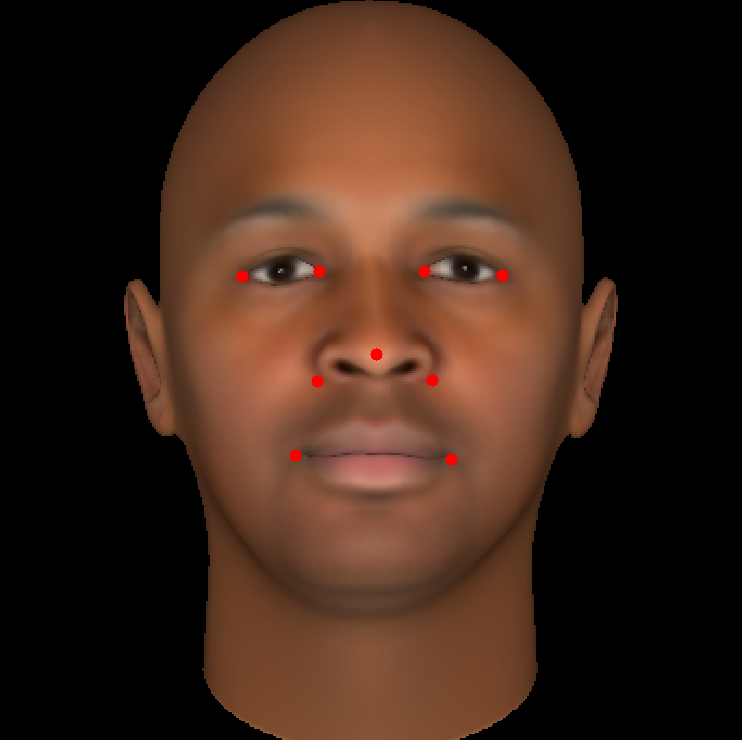
\includegraphics[width=.33\linewidth]{resources/figures/extracted_fiducial_0006.png} &
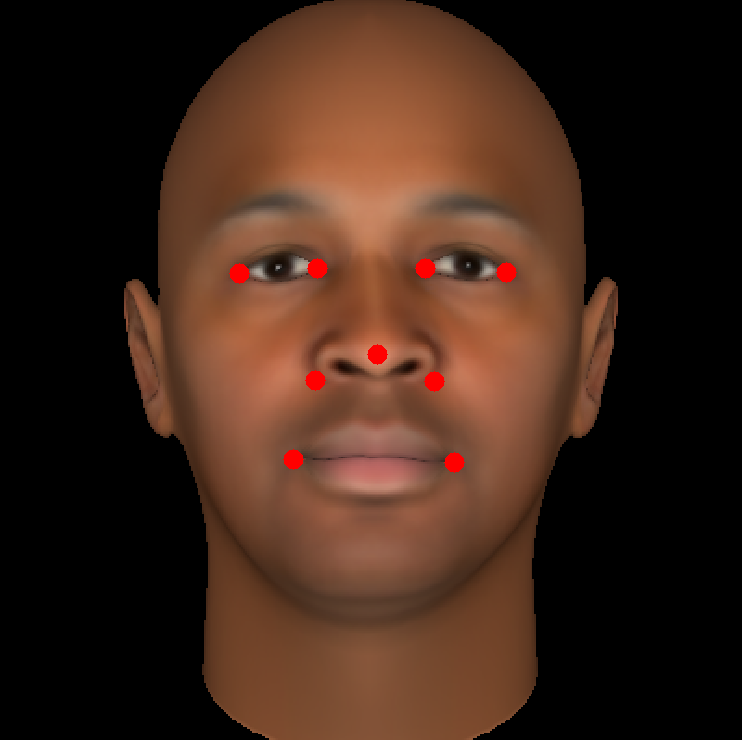
\includegraphics[width=.33\linewidth]{resources/figures/extracted_fiducial_0008.png} &
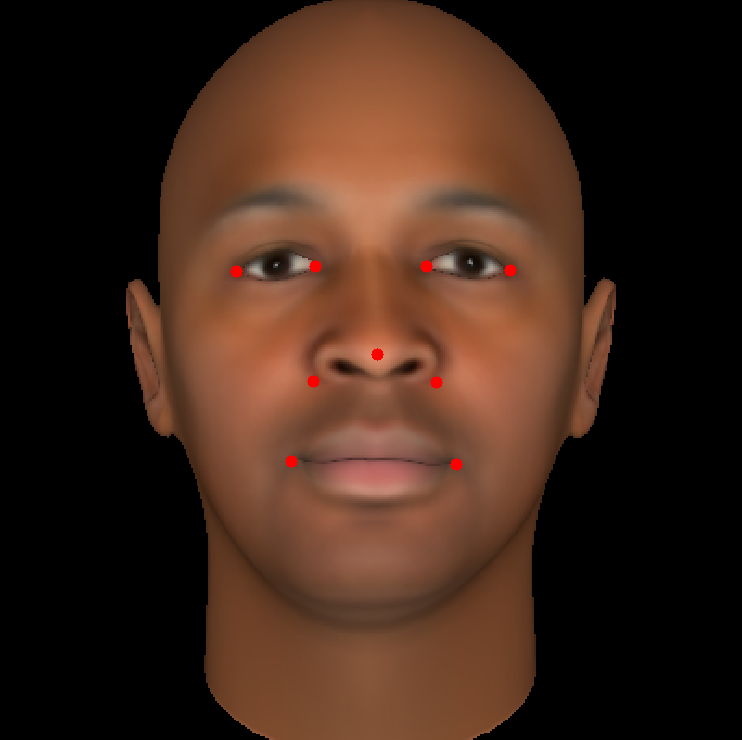
\includegraphics[width=.33\linewidth]{resources/figures/extracted_fiducial_0001.png} \\
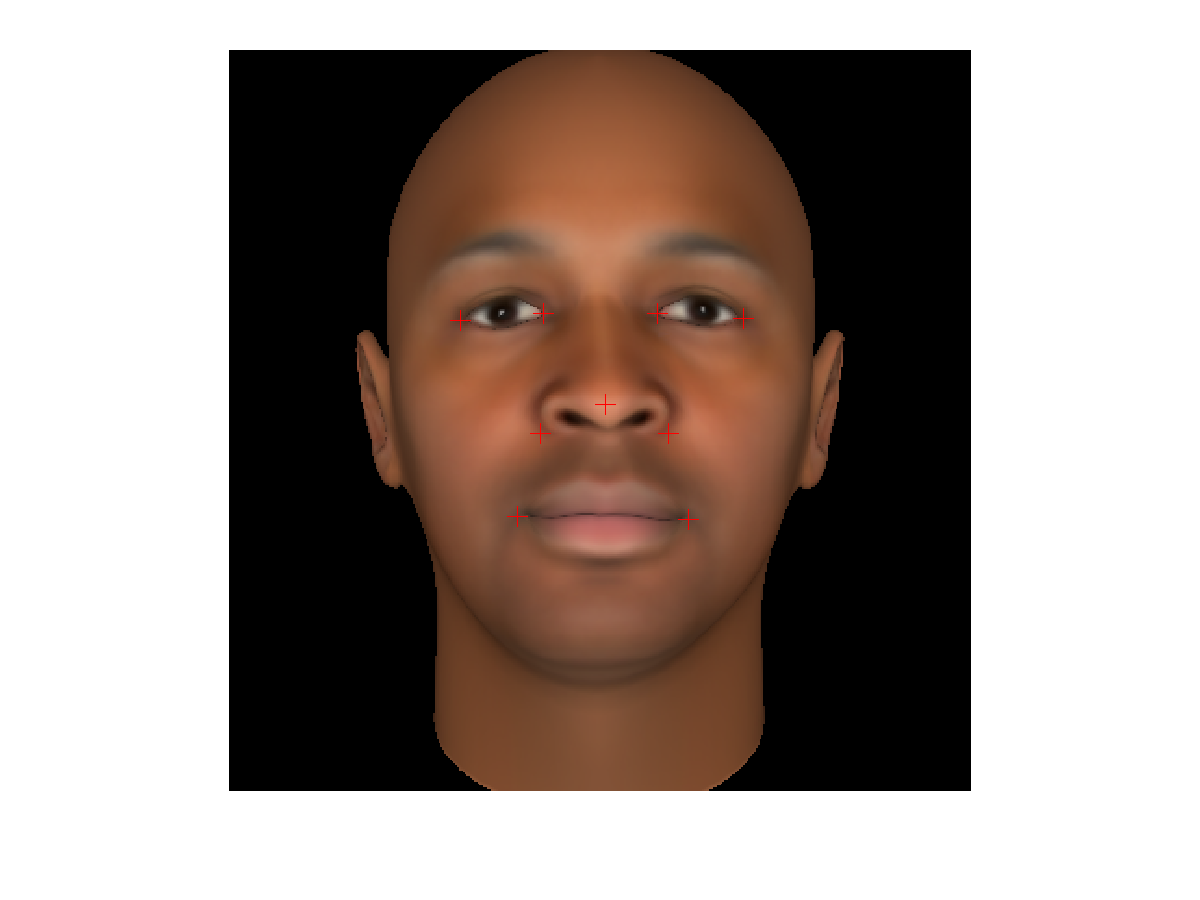
\includegraphics[width=.33\linewidth]{resources/figures/extracted_fiducial_0002.png} &
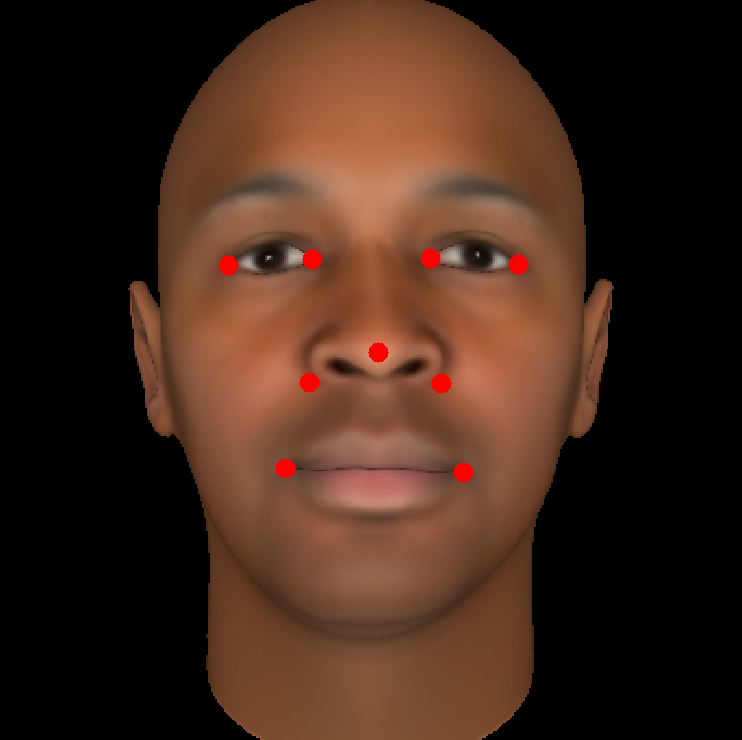
\includegraphics[width=.33\linewidth]{resources/figures/extracted_fiducial_0003.png} &
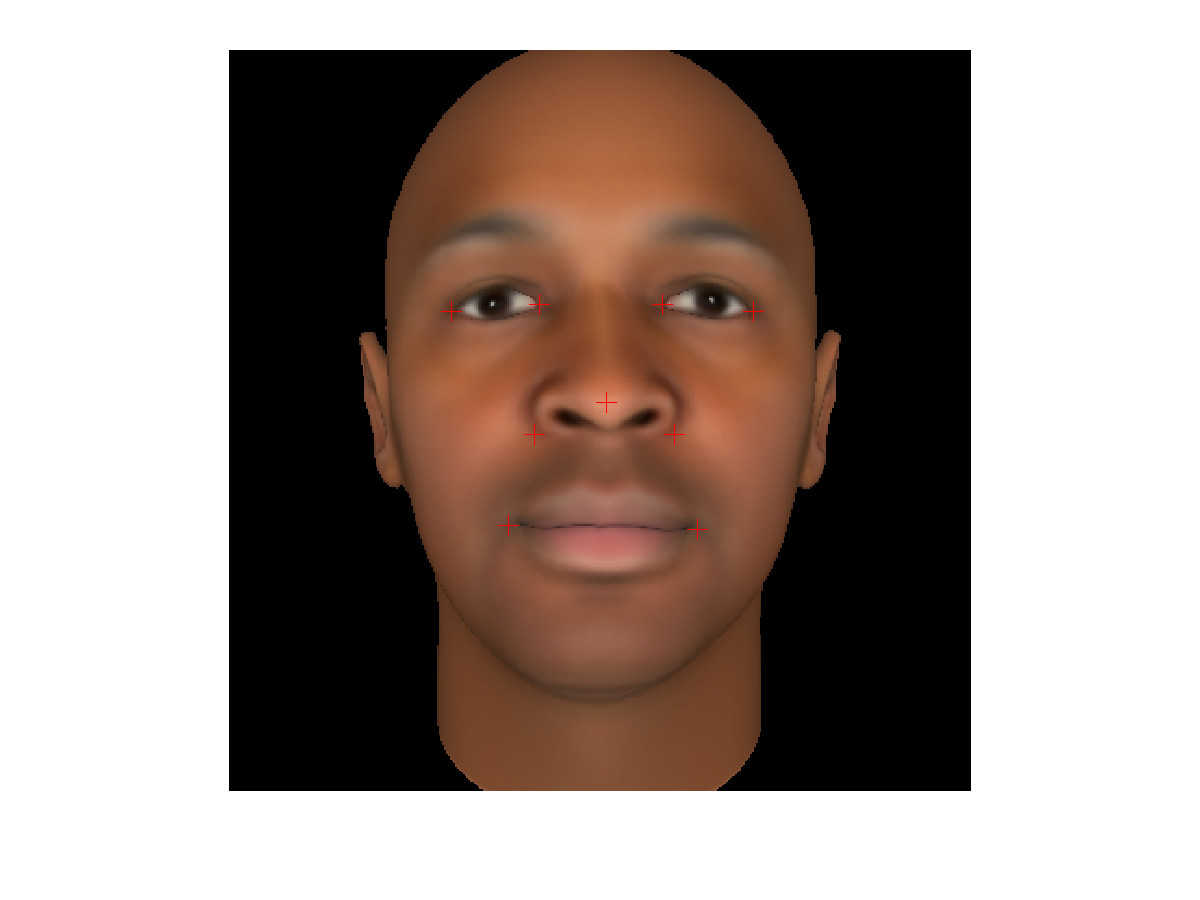
\includegraphics[width=.33\linewidth]{resources/figures/extracted_fiducial_0004.png} \\
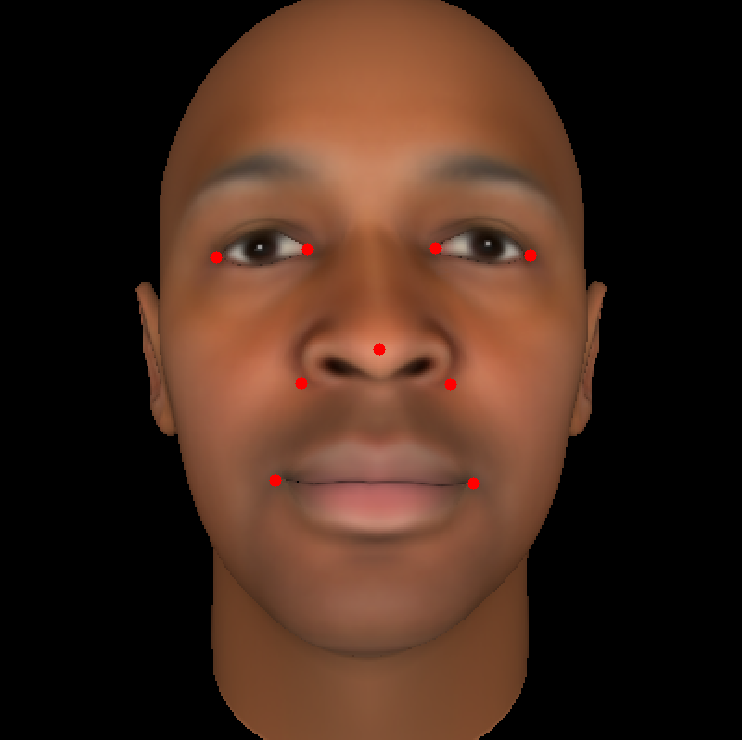
\includegraphics[width=.33\linewidth]{resources/figures/extracted_fiducial_0005.png} &
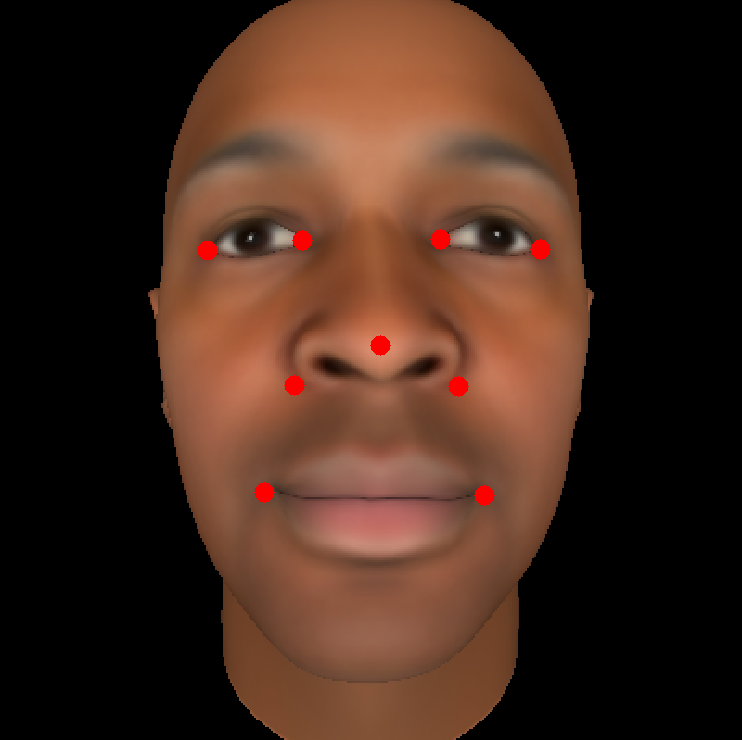
\includegraphics[width=.33\linewidth]{resources/figures/extracted_fiducial_0007.png} &
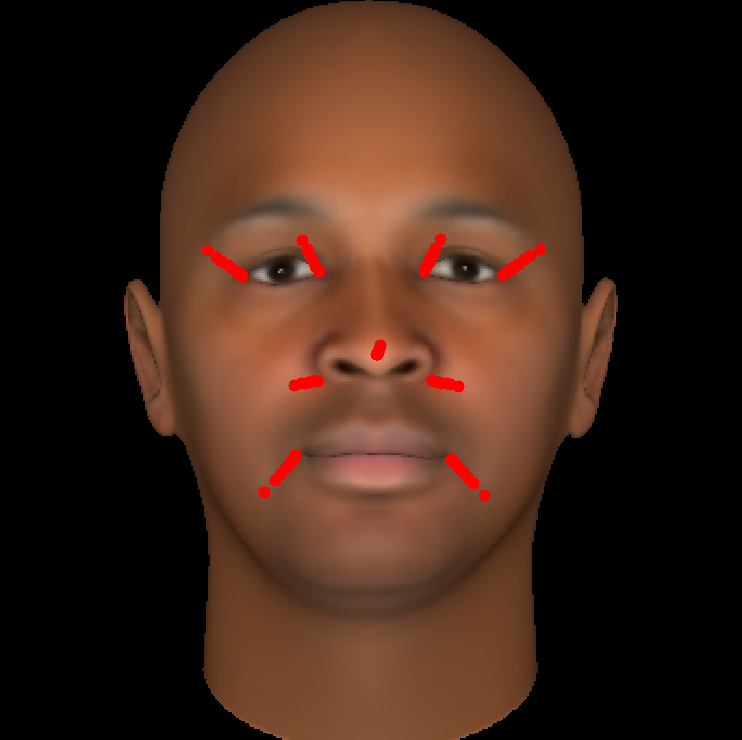
\includegraphics[width=.33\linewidth]{resources/figures/fiducial_migration.png}
\end{tabular}
\caption{
A synthetic head viewed from different camera distances, illustrating projective distortion.
Camera distance decreases in the first eight images, indexed in row-major order.
Here, the focal length (zoom) is adjusted to keep the figure at a constant size.
Fiducials are shown as red dots.
In the first image, the camera is a far distance, resulting in near orthographic projection.
In the eighth image (bottom row, middle column) the camera is very close to the human head, resulting in an elongated face and protruding nose.  
The last image is the same as the first, but with fiducial markers from all images.
This illustrates the migration of fiducials as a function of camera distance. 
} 
\label{fig:fiducial_migration}
\end{figure}

\subsection{Related works} \label{sec:related}
There is previous work on head pose estimation from 2D images; see \cite{murphy2009head} for a recent survey.
However, most methods attempt to recover a subset of the yaw, pitch, and roll of the head with respect to the camera.
To our knowledge, these methods do not attempt to estimate the distance between the camera and head; Figure \ref{fig:head_pose} illustrates the difference.
In this section we discuss works most similar to our own.

\begin{figure}[ht]
\centering
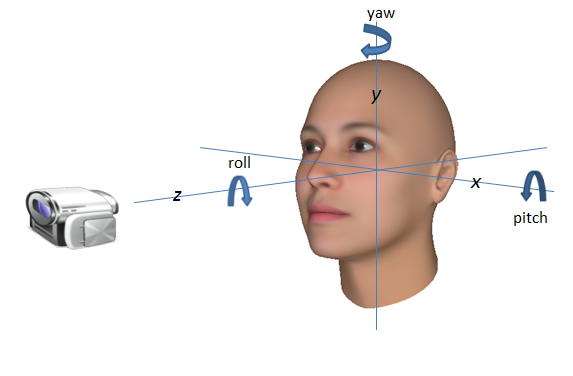
\includegraphics[width=1.0\linewidth]{resources/figures/head_pose.png}
\caption{
An illustration of the six degrees of freedom governing head pose relative to a camera.
Prior work has focused on estimation of yaw, pitch, and roll \cite{murphy2009head}.
In this paper, we assume these parameters are known and estimate camera distance from the subject, shown here as distance along the $z$ axis.
}
\label{fig:head_pose}
\end{figure}

In \cite{liu2003face,liu2006face}, Liu et al. study the effect of face recognition by humans when viewing faces at different perspective convergence angles (effectively focal length or field of view). 
The study involved a training phase in which face images were displayed to a human test subject.
In a later recognition phase the subject was shown images of faces and asked to determine whether each face had been previously displayed.
The field of view was changed to see if this had an effect on recognition. 
Their results show that even humans have a hard time recognizing a face when viewed under different levels of perspective distortion.  
This is a motivating factor since if humans have trouble with this task, a computer vision algorithm will likely also have the same troubles.  
Predicting the distance between camera and face is a first step in mitigating the effects of perspective distortion.

A similar psychology based studied is presented in \cite{perona2007new,bryan2012perspective}. 
Here, Perona et al. investigate the effects of perspective distortion as visual cue for social judgement of faces.  
Human subjects were asked to judge an image of a face in terms of trustworthiness, attractiveness, and competence.  
Their results show that for social judgements, pictures taken up close are generally rated lower, while pictures taken far away have higher ratings.

In automatic camera calibration, camera parameters are recovered using prior information about the imaged scene.
In \cite{deutscher2002automatic}, Deutscher et al. recover camera parameters under the assumption the scene satisfies a Manhattan world criterion.
This is similar to our technque, which assumes human fiducial locations are approximately distributed according to an estimated distribution. 
In \cite{lv2006camera}, Lv et al. use a human subject for calibration, but unlike this work requires multiple frames of video.
In \cite{krahnstoever2005bayesian}, Krahnstoever and Mendonca use a full human body for calibration from a single image, where this work uses just the head.

In \cite{ohayon2006robust}, Ohayon and Rivlin present head tracking as a camera pose estimation problem.  
Prior to head tracking, 3D points are acquired from the head.  
During tracking, correspondences between the 3D points and their imaged 2D points are used to estimate head pose by solving the inverse problem, namely camera pose. 
They use the Perspective $n$-Point (\PnP) formulation to solve for the camera extrinsic parameters (rotation $R$ and translation $T$).  
The \PnP~method is also known as the Location Determination Problem and was first coined in \cite{ransac}.  
In effect, the human head is used as a calibration rig.  
In this paper, the authors show that head pose can be accurately estimated and tracked under varying yaw, pitch, and roll and translations about $x$ and $y$ axes. 
However, they assume knowledge of the ground-truth fiducial locations and do not address dramatic changes in camera distance.

\section{Camera pose estimation from face images using \EPnP} \label{sec:method}

Our work is based on \cite{ohayon2006robust}, but we focus primarily on translation along the $z$-axis, which affects the level of induced perspective distortion.  
% Furthermore, Ohayon and Rivlin present a method for estimating head pose of a specific human head.  
We present a method for estimating the pose of a previously unseen human head using a dataset of exemplar human heads. 

\subsection{Efficient Perspective $n$-Point (\EPnP)}
\EPnP~is a non-iterative solution to the \PnP problem.  
As stated earlier, the \PnP~problem estimates the pose of a calibrated camera from $n$ 3D-to-2D correspondences.  
The advantage of \EPnP~is that the computational complexity grows linearly with $n$, whereas other state-of-the-art methods are $O(n^5)$ or even $O(n^8)$.  
We use Matlab code provided by the authors \footnote{\url{http://cvlab.epfl.ch/software/EPnP}}.

\subsection{Exemplar 3D heads}
The geometric configuration of fiducial features does vary from face to face, but in general fiducial locations tend to form clusters, as illustrated in Figure \ref{fig:fiducial_clusters}.  
Figure \ref{fig:fiducial_clusters}(a-c) shows point clouds of three different faces taken from the GavaBDB \cite{moreno2004gavabdb} dataset. 
Manually clicked fiducial locations are marked with large red dots.
\ericnote{Descriptions for how to interpret figures should be moved to captions.}
Figure \ref{fig:fiducial_clusters}(c) shows fiducials for 20 different faces.  Fiducials were aligned by subtracting their respective means.  
Note the fiducials form clusters.  
We take advantage of this and use a set of exemplar 3D heads to estimate the camera pose (in particular distance between camera and head) of face images in general. 
We show that using exemplar heads allows us to accurately estimate the camera pose and distance from camera to the head.

\begin{figure}[h]
\centering
\begin{tabular}{cc}
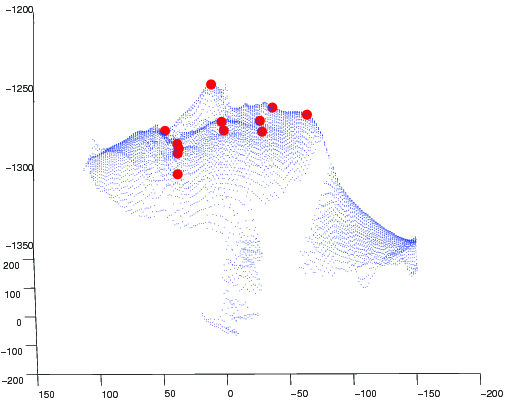
\includegraphics[width=.3\linewidth]{resources/figures/face1.png} &
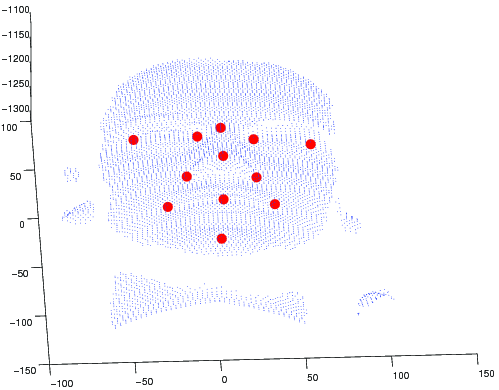
\includegraphics[width=.3\linewidth]{resources/figures/face2.png} \\
(a) & (b) \\
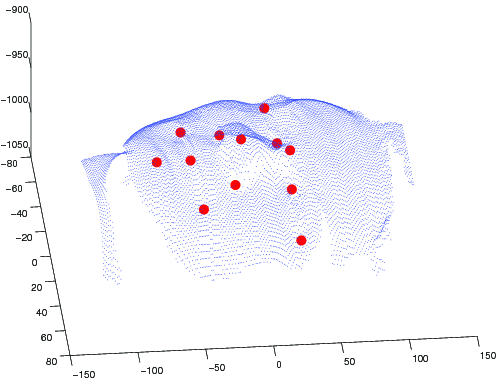
\includegraphics[width=.3\linewidth]{resources/figures/face3.png} &
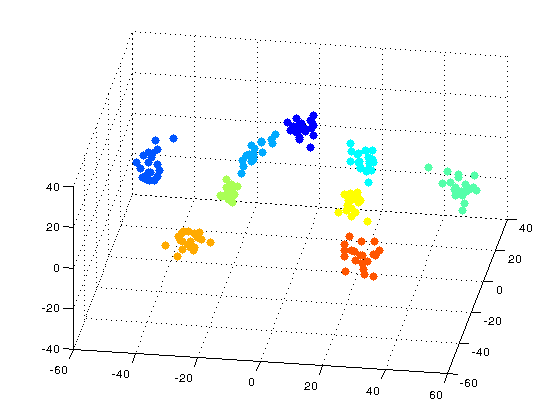
\includegraphics[width=.5\linewidth]{resources/figures/fiducial_clusters.png} \\
(c) & (d)
\end{tabular}
\caption{(a-b) 3D point clouds of three different faces along with manually clicked fiducials.  (c) Fiducials from 20 faces.}
\label{fig:fiducial_clusters}
\end{figure}

\section{Experimental setup} \label{sec:experiments}
In all experiments, we use the Texas 3D Face Recognition Database (Texas 3DFRD) \cite{gupta2010texas}, see figure \ref{fig:t3dfrd}.  
This database is a collection of 1149 pairs of frontal facial color and range images of 105 adult human subjects.  
Each face also has 25 manually labeled anthropometric facial fiducial points.  
Color and range images were captured simultaneously and are perfectly registered to each other.  
This allows us to have ground truth 3D locations of the fiducial locations.  
\begin{figure}[h]
\centering
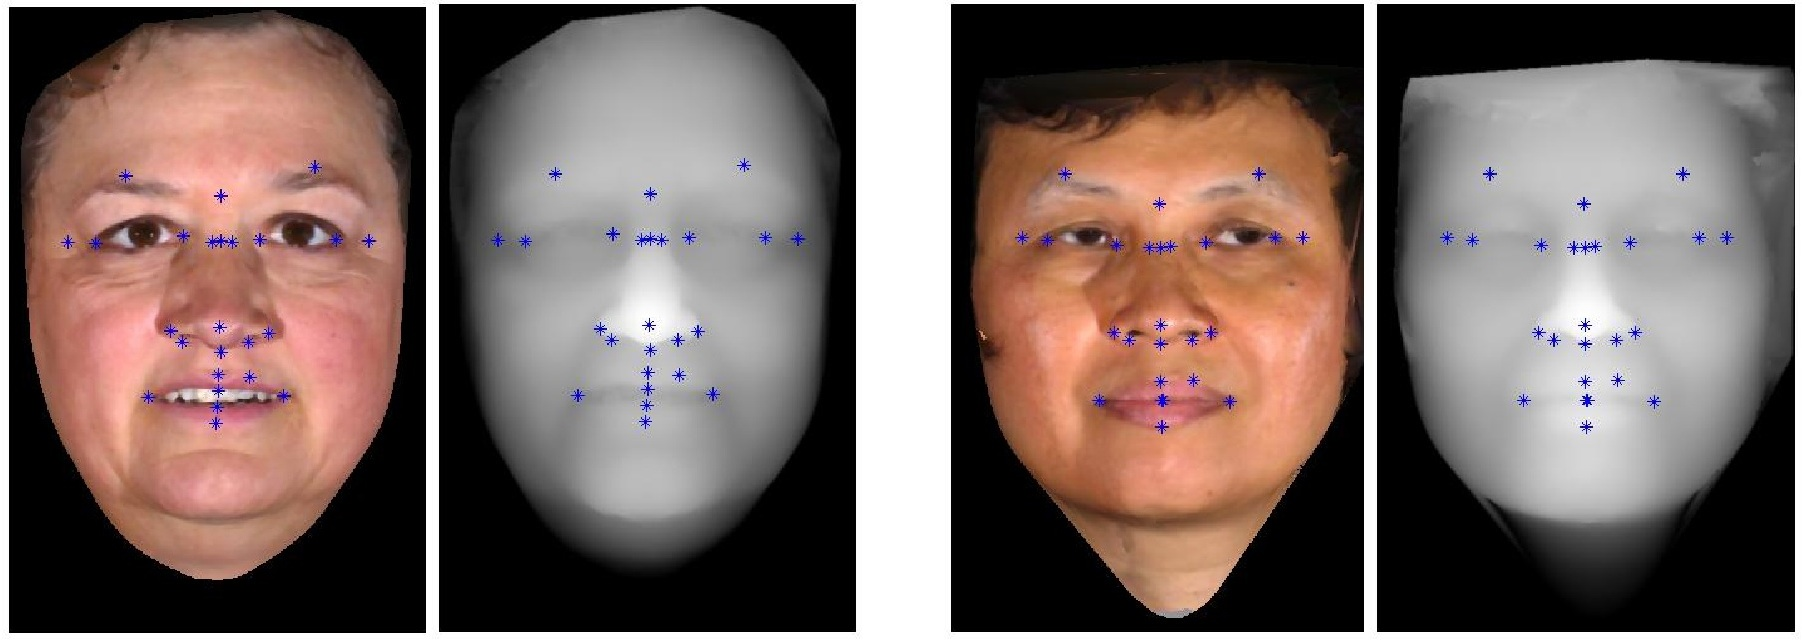
\includegraphics[width=.7\linewidth]{resources/figures/t3dfr.jpg}
\caption{Example images from the Texas 3DFRD.}
\label{fig:t3dfrd}
\end{figure}
In this work, we are primarily interested in recovering the distance between camera and head.  Our experiments consist of the following:

\begin{itemize}
\item Project fiducials for a test individual onto an image plane.
\item Use 3D fiducial locations from a set of reference individuals (not including the test individual) as exemplars.
\item For each exemplar, estimate the camera pose (and distance) using \EPnP.
\item Final estimate is the average from all exemplars.
\item Repeat while simulating a dolly-zoom (or Hitchcock zoom) camera movement (move camera back, increase focal length).  
\end{itemize}

We perform this experiment for the frontal and $3/4$ profile view of the face.  
For the frontal case, we assume all fiducials are visible to the camera.  
For the $3/4$ we assume only a subset of the fiducials are visible. 
In this work, we assume we have a calibrated camera and all intrinsic camera parameters are known.  
Simulated camera distances range from approximately $10$cm to $3$m.

Note the distance of camera to the face could be trivially estimated by the size of the imaged face if we did not adjust the focal length. 
The focal length is adjusted to keep the outermost fiducials at a near constant distance, which also keeps the imaged face silhouette at a constant size.

Figure \ref{fig:results} shows results of camera pose estimation and distance from camera to head for the frontal and $3/4$ profile views.  Figure \ref{fig:results} (a,c) qualitatively show the estimated camera pose.  The true and estimated camera distances (Figure \ref{fig:results}(b,d) )represent the distance between the camera center and tip of the nose.  The distance is reported in centimeters using an estimate for the average distance between outermost fiducial markers ($12$ cm). Note the final distance estimate closely follows the true camera distance, though the error bars get larger as the distance increases.  This is specially true for the $3/4$ profile view, presumably due to fewer number of visible fiducials.   
\begin{figure}[ht]
\begin{tabular}{cc}
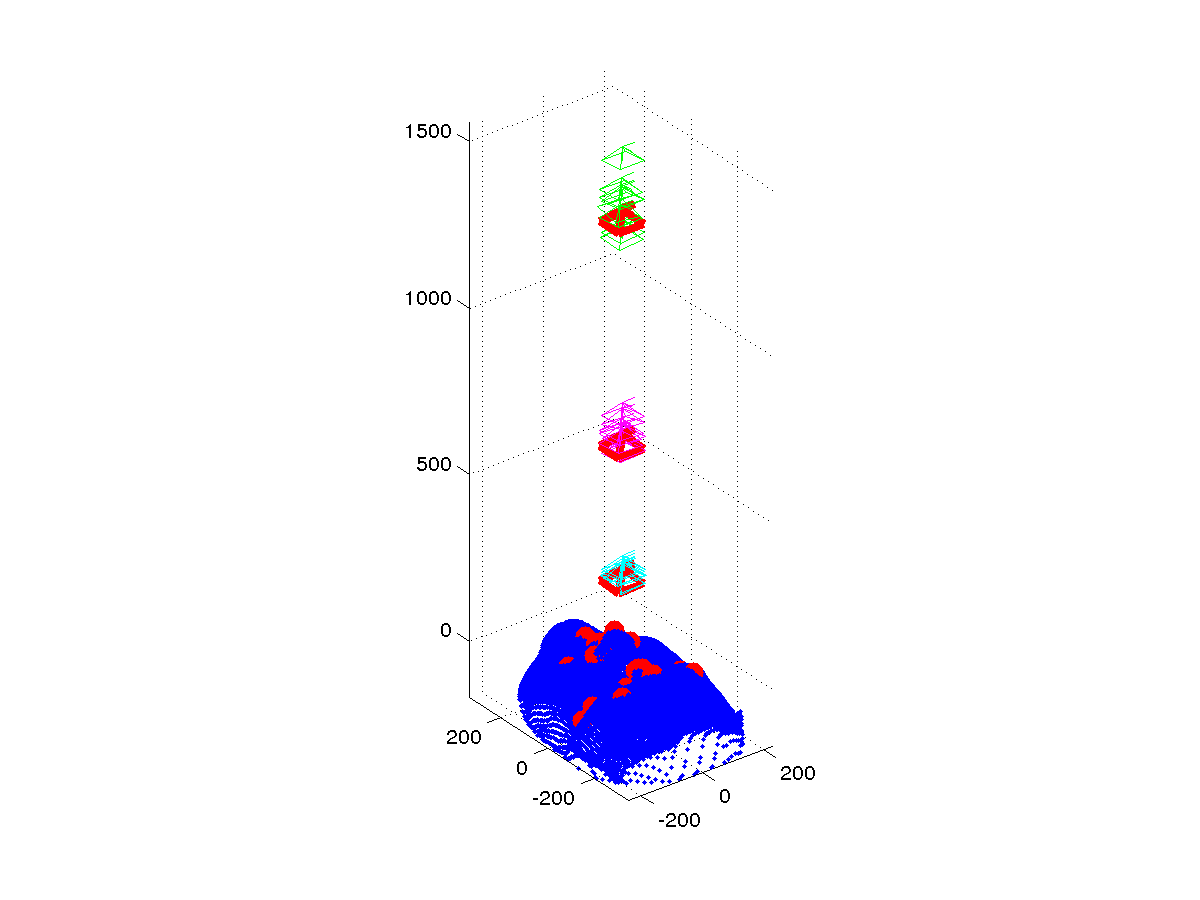
\includegraphics[width=.5\linewidth]{resources/figures/cameraloc_frontal.png} &
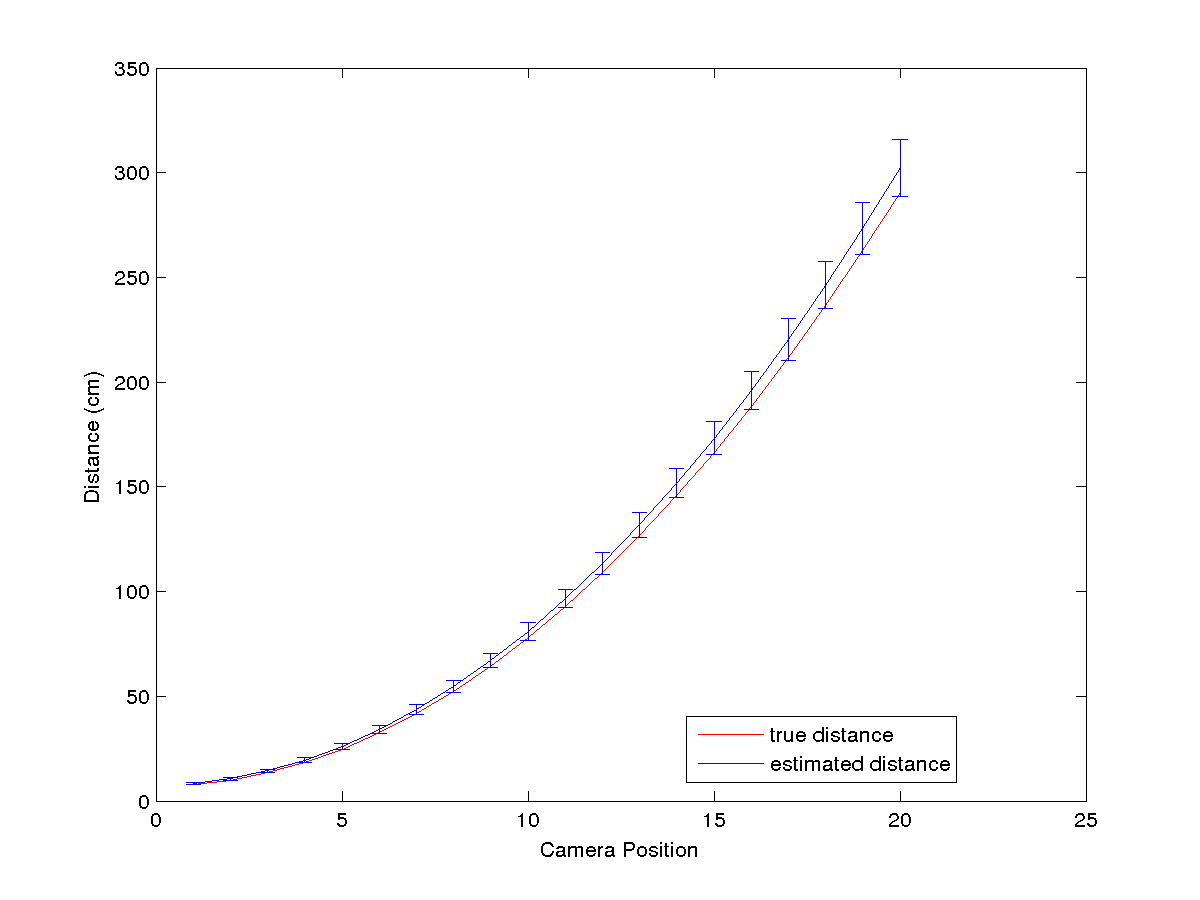
\includegraphics[width=.5\linewidth]{resources/figures/errorbar_frontal.png} \\
(a) & (b) \\
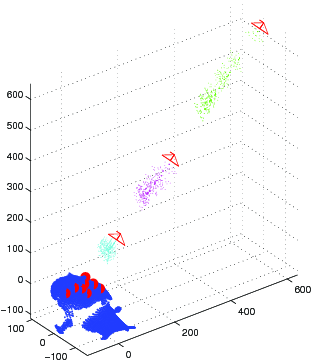
\includegraphics[width=.5\linewidth]{resources/figures/cameraloc_3q.png} &
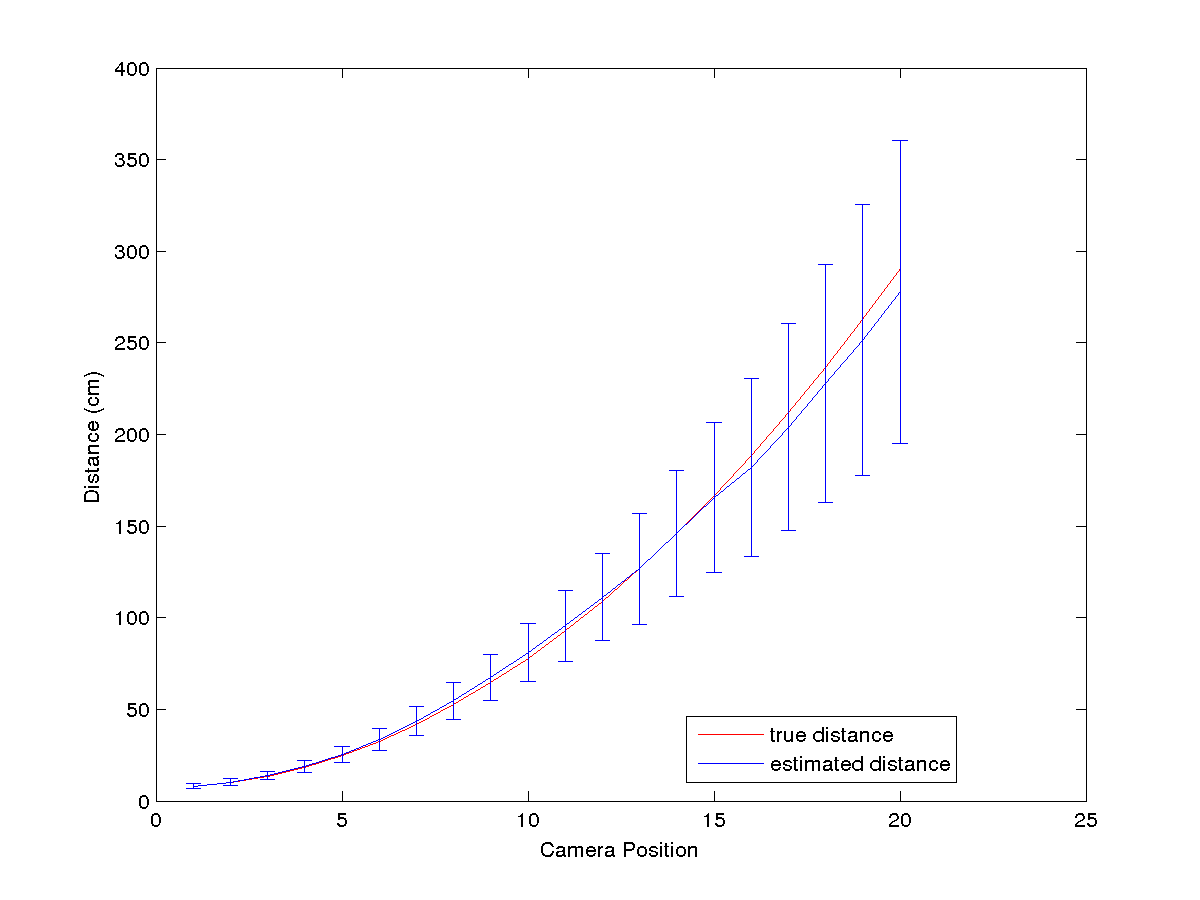
\includegraphics[width=.5\linewidth]{resources/figures/errorbar_3q.png} \\
(c) & (d)
\end{tabular}
\caption{	
(a) Camera pose estimation results for the frontal case.  
True camera position is the solid red axis.  
Estimated camera positions for near/medium/far are shown in cyan/magenta/green respectively.   
(b) Distance estimate as an average of exemplar models.  
We test $20$ camera positions and corresponding focal length to keep distance between outermost fiducials next to eye at a near constant. 
(c) and (d) show equivalent results for $3/4$ profile view.}
\label{fig:results}
\end{figure}

Figure \ref{fig:error_bar_frontal_lessfiducials} shows the same experiment with different numbers of fiducials used in the \EPnP~algorithm.  For this experiment, we manually selected the fiducial subsets to be evenly distributed about the face.  This figure shows the distance can be reliably estimated with as little as five fiducials.  In the case of five fiducials, the fiducials used were outer corners of eyes and mouth, and center of top lip.  When using only four fiducials, the center of top lip was removed, resulting in 4 nearly co-planar points.  At this point, the distance estimate becomes unreliable.

\begin{figure}[h]
\centering
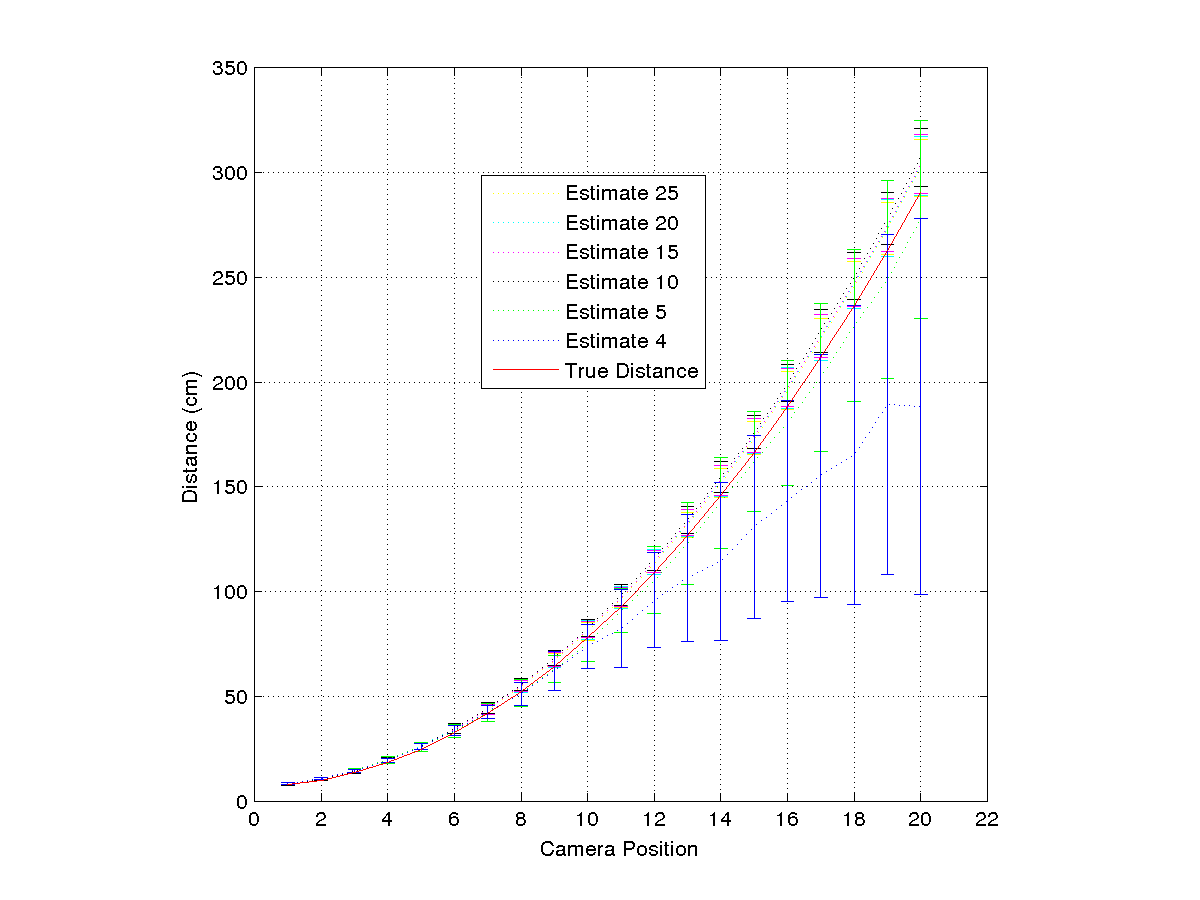
\includegraphics[width=.8\linewidth]{resources/figures/errorbar_frontal_lessfiducials.png}
\caption{Error bars of camera distance for the frontal view using different numbers of fiducials.}
\label{fig:error_bar_frontal_lessfiducials}
\end{figure}

For qualitative analysis, we use a heuristic to select a ``best'' exemplar.  Let $p_i$ be the 2D imaged fiducial using the true camera position.  
Let $p_{ij}'$ be the imaged fiducial using the estimated camera position from the $j$-th exemplar.
We use $\argmin_j \sum_i \|p_i - p_{ij}'\|$ as a heuristic to select the best exemplar. 
See Figure \ref{fig:bestexemplar} for some illustrative examples.  
In these examples, it is interesting to see what can be recovered by simply using fiducial geometry.  
Top row shows best exemplar matches the gender of the probe image.  
Second row shows similar race in two out of three cases.  
In all cases, the general shape of the image is returned in the best matching exemplar.\afbnote{add more interesting commentary here}.

\begin{figure}[h]
\centering
\begin{tabular}{cc}
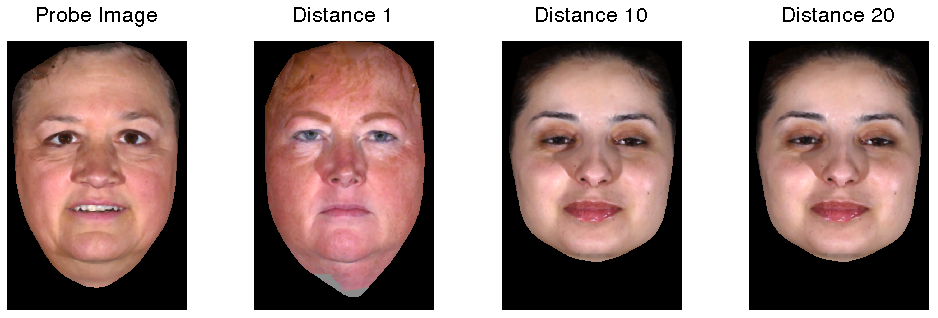
\includegraphics[width=.7\linewidth]{resources/figures/best_exemplar1.png} \\
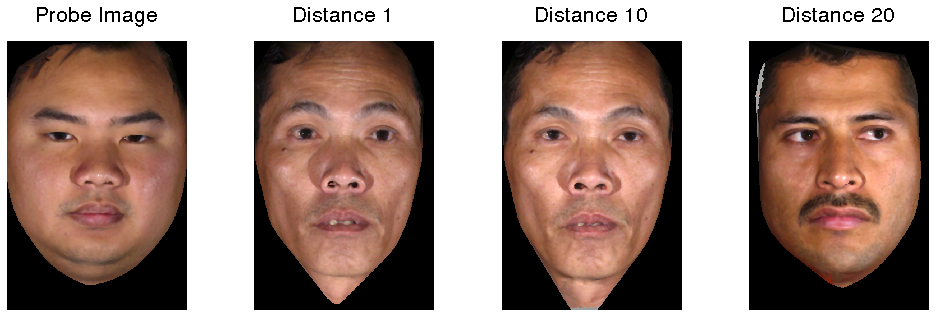
\includegraphics[width=.7\linewidth]{resources/figures/best_exemplar3.png} \\
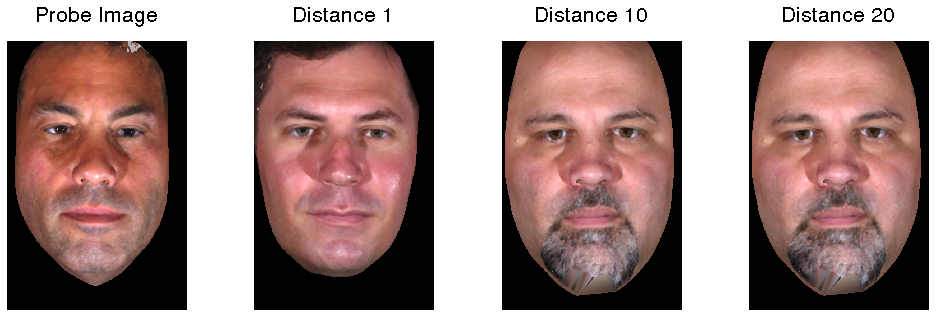
\includegraphics[width=.7\linewidth]{resources/figures/best_exemplar10.png} \\
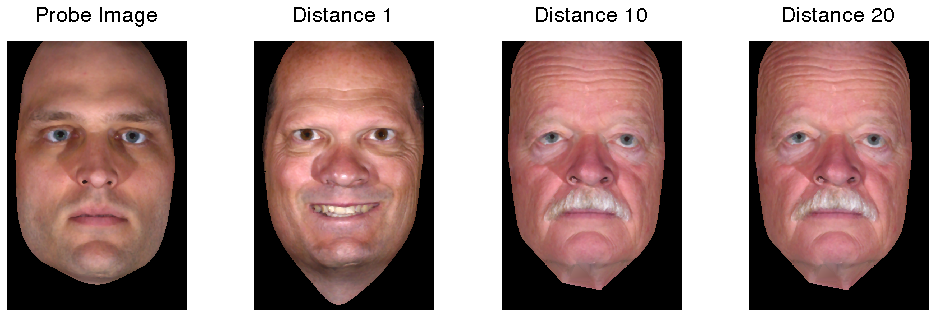
\includegraphics[width=.7\linewidth]{resources/figures/best_exemplar26.png}
\end{tabular}
\caption{Best exemplar face using a heuristic of Sum of Squared error between imaged 2d fiducial points from true camera position and estimated camera position.  In each row, left column shows a probe image followed by its best matching exemplar at different camera distances. Distances (or camera positions) one, ten, and twenty correspond to physical distances of 10cm, 75cm, and 300cm, respectively. }
\label{fig:bestexemplar}
\end{figure}

\section{Conclusion and future work} \label{sec:discussion}
We have shown a method for estimating the distance from camera to a previously unseen face using correspondences of 2D imaged fiducials to 3D fiducial locations on exemplar heads.  
The distance estimate is accurate in distances ranging from 10cm to 300 cm for the frontal and $3/4$ profile views.  
Providing an estimate of this distance can be used to mitage the effects of perspective distortion in face recognition.  

In this paper, we have used a dataset consisting of facial range images with manually labelled fiducials.    
Furthermore we assume an ideal pinhole camera model and we control the pose of both head and camera.  
This simplifies the problem since we have accurate ground truth 2D and 3D fiducial locations. 
For future work, we plan to use methods for detecting fiducials such as \cite{belhumeur2011localizing}, or naturally ocurring features (e.g. SIFT features \cite{lowe}) as in \cite{ohayon2006robust}.    

\bibliographystyle{splncs}
\bibliography{library}

\end{document}
